\textcolor{blue}{Problem 3}

9.5 Fading channel. Consider an additive noise fading channel
\begin{figure}[htbp]
    \centering
	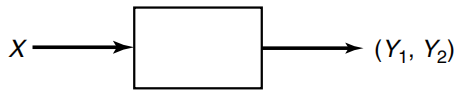
\includegraphics[width=0.4\textwidth]{../figure/9_1_9_2.png}
\end{figure}
$$ Y =XV + Z$$

where $Z$ is additive noise, $V$ is a random variable representing fading, and $Z$ and $V$ are independent of each other and of $X$. Argue that knowledge of the fading factor $V$ improves capacity by showing that
$$I(X ; Y \mid V) \geq I(X ; Y)$$

\textcolor{blue}{Solution}

From the chain rule of mutual information, we have
\begin{align*}
I(X;Y,V) &= I(X;Y) + I(X;V|Y) \\
&= I(X;V) + I(X;Y|V)
\end{align*}
Since $X\perp V$, so $I(X;V) = 0$. Therefore, we have
$$I(X;Y|V) = I(X;Y) + I(X;V|Y)$$
Since conditional mutual information is also a mutual information, which means that it has the same properties as mutual information, we have
$$I(X;V|Y)\geq 0$$
Therefore, we have
$$I(X;Y|V) \geq I(X;Y)\qed$$

\newpage